\documentclass{beamer}
 
\usepackage[utf8]{inputenc}
\usepackage{multicol}

\usetheme{Szeged}
\usecolortheme{beaver} 
 

\title{Lerntraining Software}
\subtitle{Python}
\author{Sophie Aerdker}
\institute{Ruhr-Universit\"at Bochum}
\date{Mai 2018}
 
 
 
\begin{document}
 
\frame{\titlepage}
\begin{frame}
\frametitle{Table of Contents}
	\begin{multicols}{3}
 		 \tableofcontents
	\end{multicols}
\end{frame}

\section{Overview}

\begin{frame}
\frametitle{Overview}
	Python is ...\\
	\begin{itemize}
		\item interpreted
		\item interactive 
		\item object-oriented 
		\item a beginners language!
	\end{itemize}
\end{frame}

\subsection{Setup}

\begin{frame}
\frametitle{For you at home, here \texttt{python} is already installed!}
	\begin{itemize}
		\item Check if \texttt{Python} is already installed: open a terminal and type "python"
		\item Linux:
		\item Windows:
	\end{itemize}
	Using \textit{Anaconda}:
	\begin{itemize}
		\item Linux:
		\item Windows:
	\end{itemize}
	Or use an IDE like \textit{eclipse} or \textit{Visual Studio}
\end{frame}

\section{First Steps}
\subsection{Hello World!}

\begin{frame}
\frametitle{ Hello World!}
	\begin{columns}[T]
		\begin{column}[T]{7cm}
			\begin{itemize}
				\item open an editor 
				\item type: \texttt{print "Hello World!"}
				\item save it as "HelloWorld.py" under ...
				\item open a terminal and go to your directory with cd ...
				\item type: \texttt{python HelloWorld.py}
			\end{itemize}
		\end{column}
		\begin{column}[T]{5cm}
			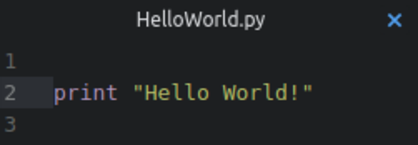
\includegraphics[width = 1\textwidth]{HelloWorld.pdf}
		\end{column}
	\end{columns}
\end{frame}

\subsection{Simple Calculations}

\begin{frame}
\frametitle{Simple Calculations}
	\begin{columns}[T]
		\begin{column}[T]{7cm}
			\begin{itemize}
				\item now type e.g. \texttt{x = 5} and \texttt{y = 10} under your print statement
				\item type \texttt{print} and a calculation using +,-,*,/
				\item save the file, go to your terminal and type \texttt{python HelloWorld.py} or press $\uparrow$
				\item What is the result of \texttt{x/y}?
			\end{itemize}
		\end{column}
		\begin{column}[T]{3cm}
			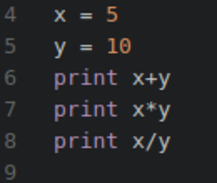
\includegraphics[width = 1\textwidth]{SimpleCalculations.pdf}
		\end{column}
	\end{columns}
\end{frame}

\section{Variable Types}

\begin{frame}
\frametitle{Variable Types}
	Python has five basic data types:
	\begin{itemize}
		\item Numbers, like 5 and 10
		\item Strings, like "Hello World!"
		\item Lists, 
		\item Dictionary, sometimes very useful but is not presented here
		\item Tuple
	\end{itemize}
	Data types can be stored in variables:
	\begin{itemize}
		\item  \texttt{x = 10}
		\item  \texttt{gravConstant = 9.81}
		\item  \texttt{s = "Hello World!"}
		\item  \texttt{name = "Sophie"}
	\end{itemize}
\end{frame}

\subsection{Numbers}

\begin{frame}
\frametitle{Basic numerical types with some examples}
	\begin{tabular}{c|c|c}
		Type & Examples & Comment \\ \hline
		int  & 3, -42 &  signed integer $ \leq 2,147,483,647$\\
		long & 51924361L & signed integer $>2,147,483,647$ \\
		float & 3.14, 3.0+e10, 0. & floating point real values \\
		complex & 42.0j, 2.+0.3j & complex numbers, imaginary unit j
 	\end{tabular}
 	
 	\begin{alertblock}{Integer Division}
 		The statement \texttt{5/10} is interpreted as an integer! Thus, its integer division is 0. Instead type 			\texttt{5./10.} to obtain a float-type value.
 	\end{alertblock}
 	\begin{block}{Boolean}
 		The result of a comparison which is \texttt{True} or \texttt{False} is called Boolean. \texttt{True} and 			\texttt{False} are special versions of 1 (or any non-zero/null value) and 0, respectively. You can use them in arithmetic contexts.
 	\end{block}	
\end{frame}

\subsection{Operators}

\begin{frame}
\frametitle{Arithmetic and Comparison Operators}
	\begin{tabular}{cc|c}
		\multicolumn{2}{c|}{Operator} & Examples  \\ \hline
		+ & Addition & 5+10 = 15  \\
		- & Subtraction & 10-5 = 5  \\
		* & Multiplication & 10*5 = 50   \\
		/ & Division & 10/5 = 2, 5/10 = 0, 5./10. = 0.5 \\
		** & Power & 10**5 = 10,000 \\
		\% & Modulus & 10\%5 = 0, 5\%10 = 5 \\
		// & Floor Division & 9.//2. = 4.0 \\ \hline
		== & equal & 5==10 is False, 5==5 is True  \\
		!= & not equal & 5!=10 is True, 5!=5 is False  \\
		$>$ & greater than & 10 $>$ 5 is True  \\
		$<$ & less than & 10 $<$ 5 is False \\
		\multicolumn{2}{l|}{$<=$ or $>=$} & 10 $>=$ 5 is True, 5 $<=$ 5 is True \\
 	\end{tabular}	
\end{frame}

\begin{frame}
\frametitle{Asignment Operators}
	\begin{tabular}{c|p{5cm}|p{3cm}}
		Operator & Description & Example  \\ \hline
		= & Assigns values from the right side to the left side & x = 5+10 \\
		+= & Adds right operand to the left one AND assigns the result to the left operand & x += 1 is equivalent to x = x + 1 \\ \hline	
		-= &  \multicolumn{2}{c}{x -= 1  is equivalent to x = x-1} \\
		*= &  \multicolumn{2}{c}{x *= 2 is equivalent to x = x*2} \\
		/= &  \multicolumn{2}{c}{x /= 2 is equivalent to x = x/2 }\\
		**= & \multicolumn{2}{c}{x **= 2 is equivalent to x = x**2} \\
		\%= &  \multicolumn{2}{c}{x \%= 2 is equivalent to x = x\%2 }\\
		//= &  \multicolumn{2}{c}{x //= 2 is equivalent to x = x//2 }\\ 	
 	\end{tabular}	
\end{frame}

\begin{frame}
\frametitle{Other Operators}
	\begin{alertblock}{Bitwise operators} 
		which perform bit by bit operations like binary AND, binary OR or shifting
	\end{alertblock}
	\begin{alertblock}{Logical operators} 
		\texttt{not} , \texttt{or} , \texttt{and} \\
	\end{alertblock}
	\begin{alertblock} {Membership operators} 
		\texttt{in} and \texttt{not in} \\test the membership in a \textit{sequence} such as lists or strings
	\end{alertblock}
	\begin{alertblock}{Identity operators} 
		\texttt{is} and \texttt{is not} \\compare the memory locations of two objects, you can often use them like \texttt{==} and \texttt{!=}	for example in \textit{if-statements}
	\end{alertblock}
\end{frame}

\subsection{Strings}

\begin{frame}
\frametitle{Strings and string formatting}
	\begin{itemize}
		\item In Python there is no difference between 'chars' and "strings", single and double quotes are treated the same.
		\item You can create strings simply by putting characters in quotes: str = \texttt{"Hello World!"}
	\end{itemize}
	You can format strings using the string formatting operator '\%': \\
	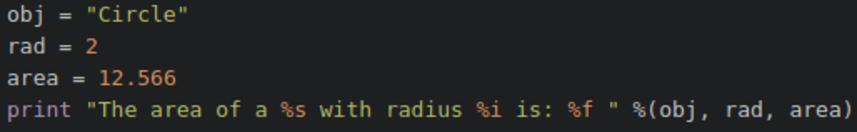
\includegraphics[width = 0.9\textwidth]{StringFormat.pdf} \\
	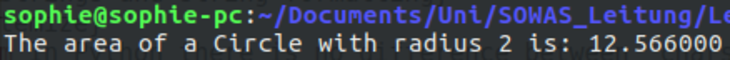
\includegraphics[width = 0.8\textwidth]{StringFormatOutput.pdf}
	
	You can find a table with format symbols here: \url{https://www.tutorialspoint.com/python/python_strings.htm}
\end{frame}


\section{Decision Making}

\begin{frame}
\frametitle{If-statements}
	\begin{columns}[T]
	\begin{column}[T]{5cm}
			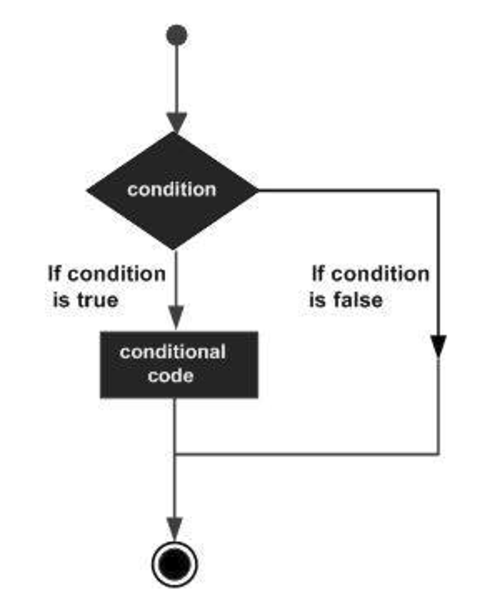
\includegraphics[width = 1\textwidth]{DecisionMaking.pdf}
		\end{column}
		\begin{column}[T]{3cm}
			use \texttt{if} and \texttt{else} conditions to execute a specific code if a condition is TRUE or to jump to the next (or another conditional) code otherwise	
		\end{column}	
	\end{columns}
\end{frame}

\begin{frame}
\frametitle{Example}
	\begin{columns}[T]
		\begin{column}[T]{0.6\textwidth}
			Some \texttt{if}, \texttt{elif}, \texttt{else} statements to compare the values x and y:\\
			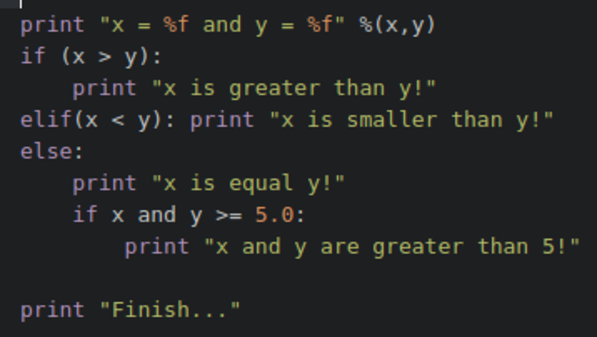
\includegraphics[width = 1\textwidth]{Comparison.pdf}
		\end{column}
		\begin{column}[T]{0.4\textwidth}
			Output for different values of x and y:\\
			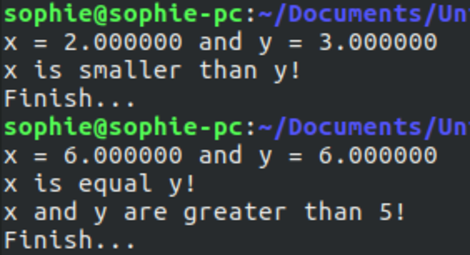
\includegraphics[width = 1\textwidth]{OutputComparison.pdf}	
		\end{column}	
	\end{columns}
	\begin{alertblock} {Syntax} 
		The conditional code has to be intended or stands in a line (only possible for one statement) with the condition. IDEs and many editors do this automatically.
	\end{alertblock}
\end{frame}


\section{Exercises}

\begin{frame}
\frametitle{Exercises}
	\begin{itemize}
		\item Write the program \texttt{EvenOdd.py} which returns wether a variable is even or odd! \\ Use operators and condition statements and print the value as well as the result!
		\item Write the program \texttt{CharInString.py} which returns wether the string \texttt{"Hello World!"} contains a specific letter (a so called char)! \\ Use membership operators and the program should be case sensitive to keep it simple.
		\item Bonus: Use a string method (\url{https://www.tutorialspoint.com/python/python_strings.htm}) to make \texttt{CharInString.py} case insensitive
	\end{itemize}
\end{frame}


\section{Lists}

\begin{frame}
\frametitle{Lists}
	A list contains several items like strings or numbers, you can easily create a list with [] and ,-separated items: 
	\begin{itemize}
	\item \texttt{fruits = ["apple", "banana", "strawberry"]}
	\item \texttt{numbers = [1,1,2,3,5,8]}
	\end{itemize}
	The items in a list can be of different types:
	\begin{itemize}
	\item \texttt{book = ["title", "physics", 1997]} 
	\end{itemize}
	You can access an item in a list by its index:
	\begin{columns}[T]
	\begin{column}[T]{5cm}
		\begin{itemize}
			\item \texttt{fruits[1]} is \texttt{"banana"} 
			\item \texttt{numbers[3]} is \texttt{3}
		\end{itemize}
	\end{column}
	\begin{column}[T]{5cm}
		\begin{itemize}
			\item \texttt{fruits[0]} is \texttt{"apple"} 
			\item \texttt{numbers[-1]} is \texttt{8}
		\end{itemize}
	\end{column}
	\end{columns}
	\begin{alertblock}{Index}
	The index of a list starts with 0! You can use negative indices, too!
	\end{alertblock}
\end{frame}

\begin{frame}
\frametitle{Manipulating Lists}
	You can use the index to change an item at the index position:
	\begin{itemize}
	\item \texttt{fruits[0] = "mango"} results in \texttt{["mango", "banana", "strawberry"]}
	\end{itemize}
	You can delete an item at a specific position:
	\begin{itemize}
	\item \texttt{del fruits[0]} results in \texttt{["banana", "strawberry"]}
	\end{itemize}
	List slicing with ':' :
	\begin{itemize}
	\item \texttt{numbers[1:4]} results in \texttt{[1,2,3]}
	\item \texttt{numbers[2:]} results in \texttt{[2,3,5,8]}
	\end{itemize}
	Merge lists:
	\begin{itemize}
	\item \texttt{numbers} + [13,21,34] results in \texttt{[1,1,2,3,5,8,13,21,34]}
	\end{itemize}
\end{frame}

\begin{frame}
\frametitle{Sequences}
	\begin{alertblock}{Strings}
		Lists and Strings both are sequences, thus accessing substrings and slicing strings works the same way!
	\end{alertblock}
\end{frame}

\begin{frame}
\frametitle{List methods}
	There are some useful methods for lists:
	\begin{itemize}
	\item \texttt{len(fruits)} returns the length of the list: 3
	\item \texttt{max(numbers)} returns the maximum value: 8
	\item \texttt{min(numbers)} returns the minimum value: 1
	\item \texttt{list.sort([func])} sorts the list \texttt{list}, using an optional sort function
	\item \texttt{list.count(obj)} returns how often \texttt{obj} occurs in \texttt{list}
	\item \texttt{list.append(obj)} appends \texttt{obj} to \texttt{list}
	\item \texttt{list.remove(obj)} remove \texttt{obj} at any position from \texttt{list}
	\end{itemize}
	You can find more methods and their decription on \url{https://www.tutorialspoint.com/python/python_lists.htm} or in the python documentation
\end{frame}

\section{Loops}

\begin{frame}
\frametitle{for-loops}
	If you want to repeat a statement while a specific condition is True, you can use loops:
	\begin{itemize}
		\item \texttt{while}-loops: \\ repeats one or more statements while a condition is true; the condition is tested before executing the conditional code
		\item \texttt{for}-loops: \\ iterates over the items of any sequence like strings or lists and executes the conditional code
	\end{itemize}
\end{frame}

\begin{frame}
\frametitle{Examples}
	
	for-loop over a list:\\
		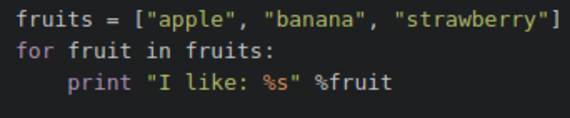
\includegraphics[height = 1.4cm]{forLoop.pdf} $\,$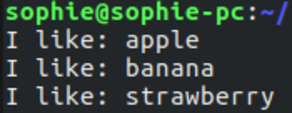
\includegraphics[height = 1.4cm]{forLoop_Output.pdf}\\
	while-loop: \\
		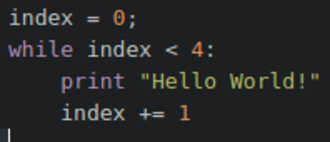
\includegraphics[height = 1.6cm]{whileLoop.pdf}$\,$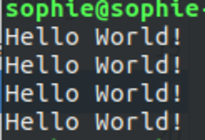
\includegraphics[height = 1.6cm]{whileLoop_Output.pdf}
	
\end{frame}
\begin{frame}
\frametitle{Examples}
	
	for-loop using \texttt{range()}:\\
		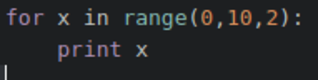
\includegraphics[height = 1.3cm]{forLoopRange.pdf} $\,$
		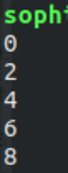
\includegraphics[height = 2cm]{forLoopRange_Output.pdf} \\
	The \texttt{range()} method creates a list with the parameters \texttt{(begin, end, step)}, where the end-value is not included! Default values are: \texttt{begin = 0} and \texttt{step = 1}, thus \texttt{range(4)} wohuld create the list \texttt{[0,1,2,3]}.
		
	
\end{frame}

\section{Exercises}

\begin{frame}
\frametitle{Exercises}
	\begin{itemize}
		\item Write the program \texttt{Faculty.py} that calculates the faculty of a certain number!
		\item Write the program \texttt{FibonacciSeries.py} that returns the Fibonacci Series! Use a list to store your result beginning with \texttt{Fibonacci = [0,1]}, the series should not exceed 10,000.
		\item Calculate the sum of all even numbers in your Fibonacci Series! You can reuse your code from exercise one.
	\end{itemize}
	There are many more mathematical problems or "number games" on \url {https://projecteuler.net/archives} you can solve with the few programming skills (but sometimes a lot of logical thinking) you have achieved here!
\end{frame}

\section{Functions}

\begin{frame}
\frametitle{Functions}
	You can organize code, that performs a single action with help of functions. This makes your code more readable and reusable. \\ You already saw a lot of "build-in" functions, like the \texttt{print} statement or the methods to manipulating lists, like \texttt{max()}. \\\ You can easily define your own functions using the \texttt{def} keyword:\\
		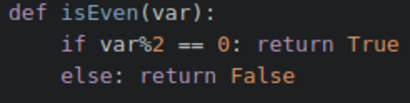
\includegraphics[height = 1.3cm]{isEvenFunc.pdf}\\
	Calling a function: \\
		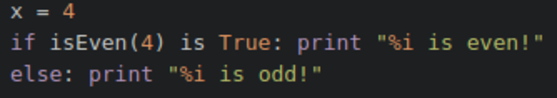
\includegraphics[height = 1.3cm]{FunctionUse.pdf}	 
\end{frame}

\section{Exercises}

\begin{frame}
\frametitle{Exercises}
	\begin{itemize}
		\item Rewrite your \texttt{Faculty.py} program with a function \texttt{faculty(n)}!
		\item Write the function \texttt{faculty(n)} \textit{recursive}. This means that the function calls itself! Take care of defining an end condition (like \texttt{faculty(0)} returns 1) , otherwise you get stuck in an infinite loop! \\
		\begin{columns}[T]
		\begin{column}[T]{6cm}
			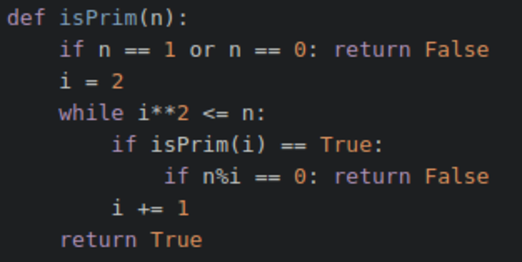
\includegraphics[width = 1\textwidth]{recursivePrim.pdf}
		\end{column}
		\begin{column}[T]{4cm}
			Example: \\
			Recursive function to calculate wether n is prime! But: this is not really efficient.
		\end{column}
		\end{columns}
	\end{itemize}
\end{frame}

\section{Modules}

\begin{frame}
\frametitle{Modules}
	For the purpose of organize and reuse your code you can create \textit{Modules} which are basically files containing Python code like functions, variables or \textit{classes}. You can \textit{import} such modules (or single functions) using the \texttt{import} statement:
	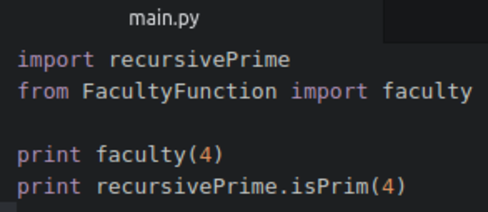
\includegraphics[width = 0.5\textwidth]{ImportStatements.pdf}
	\begin{alertblock}{Directory path}
		Your main method and modules must be in the same directory or you have to define a PYTHONPATH.
	\end{alertblock}
\end{frame}
	
	\subsection{Namespaces}
	
\begin{frame}
\frametitle{Namespaces}
	\begin{columns}[T]
		\begin{column}[T]{5.5cm}
			To avoid typing the module name before each function you imported with the \texttt{import} statement or to confuse different functions with similar names, you can use \textit{namespaces}. \\ Or you can import all items from one module into the current namespace using * (although this is not recommended and should be used  wisely)
		\end{column}
		\begin{column}[T]{5cm}
			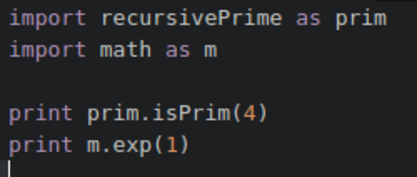
\includegraphics[width = 1\textwidth]{Namespaces.pdf} \\
			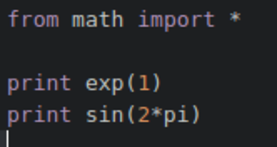
\includegraphics[width = 0.8\textwidth]{StarImport.pdf}
		\end{column}
		\end{columns}
\end{frame}

	\section{Command Line Arguments}

\begin{frame}
\frametitle{Command Line Arguments}
	For a convenient use of your programs you wouldn't want to open your python file, change the variables, save the file and then run it over the command line. Instead it would be better to run the code and define the variables over the command line: \\ $\,$ \\
	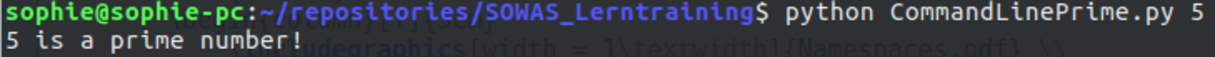
\includegraphics[width = 1\textwidth]{CommandLinePrime.pdf} \\
	This works with the \texttt{sys}-module you can easily import. This system module provides the list \texttt{sys.argv} which contains command line arguments as strings. \\ Another way is to read the keyboard input during runtime of your program using the \texttt{raw\_input} or \texttt{input} methods.
\end{frame}

\subsection{sys module}

\begin{frame}
\frametitle{sys-module example}
	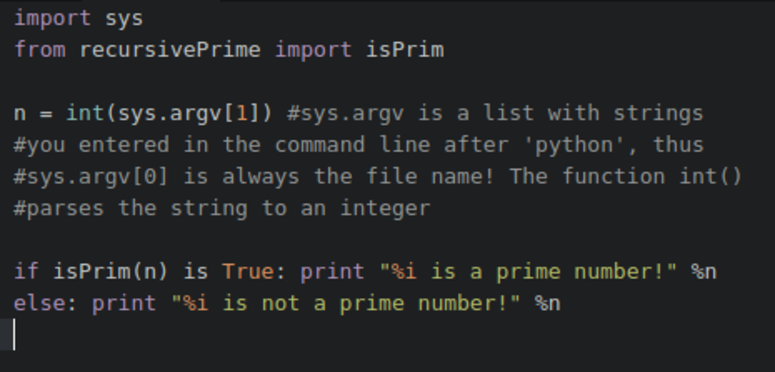
\includegraphics[width = 1\textwidth]{SysExample.pdf} 
\end{frame}

\section{Exercise}

\begin{frame}
\frametitle{Exercises}
	\begin{itemize}
		\item Write a new command line based faculty program using the sys module! Import your old \texttt{faculty} function to calcuate it!
		\item Import the math module, and do some random calculation using its member functions. You can find them in the python documentary: \url{https://docs.python.org/2/library/math.html}
	\end{itemize}
\end{frame}

\section{Files}

\begin{frame}
\frametitle{Opening and closing files}

\end{frame}
\begin{frame}
\frametitle{Reading and writing files}

\end{frame}

\section{Matplotlib}
\begin{frame}
\frametitle{Matplotlib}

\end{frame}


\end{document}